%%%%%%%%%%%%%%%%%%%%%%%%%%%%%%%%%%%%%%%%%%%%%%%%%%%%%%%%%%%%%%%%
\chapter{Introduction}
\setcounter{figure}{0}
\setcounter{table}{0}
\setcounter{equation}{0}

\minitoc

\clearpage
Les détections de plusieurs milliers d'exoplanètes sont actuellement confirmées grâce à de multiples méthodes de détection. Les méthodes de détection indirectes sont celles qui ont été les plus fructueuses pour détecter de nouvelles planètes mais, contrairement aux méthodes de détection directes, elle ne permettent pas (ou peu) la caractérisation chimique et astrométrique des exoplanètes. En effet, pour cela il s'agit de concevoir des instruments atteignant des hautes performances en terme de résolution angulaire et de contraste afin de détecter la lumière provenant directement de la planète.

La technique de masquage et de réarrangement de pupille à l'aide de fibres optiques monomodes permet de relever à la fois ces deux défis techniques et de permettre la caractérisation spectroscopique des systèmes observés. L'instrument \ac{FIRST} l'implémentant a montré par le passé ses capacités de haute résolution angulaire pour la caractérisation de binaires d'étoiles \citep{huby2013}. Mon travail de thèse s'inscrit dans la volonté d'améliorer les performances en contraste de cet instrument en intégrant la technologie d'optique intégrée.

Dans cette partie j'introduirai donc le contexte de l'étude des exoplanètes, les solutions techniques existantes et les apports des techniques de masquage et de réarrangement de pupille. Je présenterai le développement de \ac{FIRST} et l'apport de \ac{FIRSTv2}. J'exposerai enfin le contexte de l'objectif scientifique dans lequel ce dernier s'inscrit : l'étude des protoplanètes.


%%%%%%%%%%%%%%%%%%%%%%%%%%%%%%%%
\section{Imagerie haut contraste et haute résolution angulaire pour l'étude des exoplanètes}

%%%%%%%%%%%%%%%%
\subsection{L'étude des exoplanètes}

Depuis la première détection d'une exoplanète, 51 Peg b \citep{mayor1995}, en (l'an de grâce) $1995$, les techniques de détection et de caractérisation de systèmes exoplanétaires n'ont cessé de gagner en sensibilité et de se diversifier. Les détections de plus de $5\,000$ exoplanètes sont confirmées à ce jour et la figure~\ref{fig:ExoplanetDetection} présente une partie de ces détections (celles dont le demi-grand axe a pu être mesuré), pour les quatre techniques de détection par vitesse radiale (cercle orange), par transit (triangle vert), par micro-lentille gravitationnelle (point violet) et par imagerie directe (carré bleu). La masse (en unité de masse de Jupiter) de l'exoplanète est tracée en fonction de son demi-grand axe en \ac{AU} ou \ac{UA}, en français. Les huit planètes du système solaire y sont aussi représentées pour comparaison, par la première lettre de leur nom dans une bulle. Enfin, seul les corps ayant une masse inférieure à $13 \,$\MJ (correspondant à la limite différenciant une planète d'une étoile selon l'\ac{IAU} \citep{lecavelierdesetangs2022}) sont représentés, ce qui induit un plafonnement horizontal des corps détectés en haut du graphique.

\begin{figure}[ht!]
    \centering
    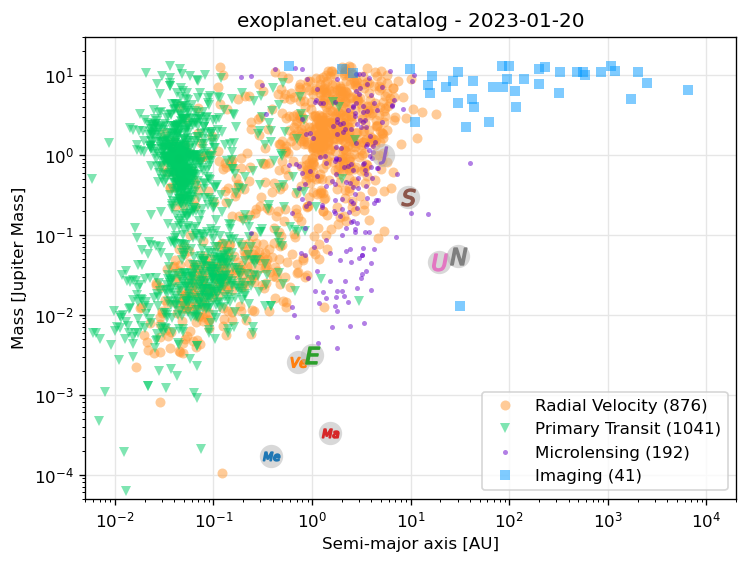
\includegraphics[width=\figwidth]{Figure_Chap1/20230120_exoplanet_diagram_RV_PT_ML_IM.png}
    \caption[Graphique des exoplanètes détectées à ce jour suivant les quatre techniques de détection principales.]{Graphique de la masse mesurées des exoplanètes détectées à ce jour en fonction de leur demi-grand axe estimé. Les détections sont identifiées par les techniques de détection par vitesse radiale (cercle orange), par transit (triangle vert), par micro-lentille gravitationnelle (point violet) et par imagerie directe (carré bleu). Seules $2\,150$ exoplanètes, dont le demi-grand axe est mesuré, sont affichées. Données tirées de la base de données de \textit{exoplanet.eu} (\url{http://exoplanet.eu/}).}
    \label{fig:ExoplanetDetection}
\end{figure}

On remarque que les deux techniques de transit et de vitesse radiale (méthode qui détecte pour la première fois 51 Peg b) ont permis de détecter la majorité des exoplanètes. Cela s'explique par le fait qu'elles sont les plus simples techniquement à implémenter en comparaison des autres. Les missions spatiales Kepler \citep{borucki2010} et \ac{TESS} \citep{ricker2016} ont ainsi été lancées afin de détecter et étudier de nouvelles exoplanètes par la méthode des transits. Ces deux missions ont permis de détecter plus de $2\,700$ et $300$ (pour $6\,000$ candidats) nouvelles exoplanètes, respectivement.

De plus, on remarque que chaque technique de détection découvre une population d'exoplanètes qui sont homologues en terme de masse et de demi-grand axe, se traduisant sur le graphique par un regroupement des points par technique de détection avec peu de chevauchement. En effet, la méthode des transits mesure la variation d'intensité lumineuse de l'étoile due au passage du compagnon en premier plan, ce qui favorise la détection des systèmes qui ont un petit demi-grand axe car cela augmente le nombre de passages et les chances que le compagnon passe entre l'étoile et la Terre. La méthode des vitesses radiales mesure le déplacement de l'étoile dans la ligne de visée et ce déplacement est d'autant plus élevé que le compagnon est massif ou que le compagnon est plus proche de l'étoile lorsqu'il est moins massif. La méthode d'imagerie consistant en l'observation de la lumière provenant du compagnon, est plus sensible aux systèmes avec une grande séparation et dont l'exoplanète est très massive (voir plus de détails dans la section~\ref{sec:ImagerieDirecte}) : elle réfléchit alors plus de lumière de son étoile ou émet un rayonnement de plus forte intensité lorsque c'est une exoplanète de type Jupiter chaude nouvellement formée. Enfin, la méthode de micro-lentille gravitationnelle qui consiste à détecter l'augmentation du flux lumineux d'une étoile en arrière-plan par l'effet de lentille gravitationnelle du compagnon d'un système exoplanétaire en avant-plan, est sensible pour une séparation idéale avec l'étoile qui ne peut ni être trop petite car on ne pourrait pas discerner l'effet de lentille de l'étoile de celui du compagnon, ni trop grande car les chances qu'à la fois l'étoile et le compagnon passent devant l'étoile d'arrière-plan sont faibles.

Par conséquent, il est nécessaire de garder à l'esprit que l'exploration de l'espace des paramètres des exoplanètes détectées est limitée et biaisée selon la méthode de détection utilisée. Cela motive l'amélioration des technologies existantes et la recherche de nouvelles solutions techniques afin d'accéder à des cas différents d'exoplanètes pour diversifier l'ensemble de nos connaissances sur les systèmes planétaires. L'imagerie directe a encore peu exploré cet espace des paramètres et se révèle très intéressante en ce qu'elle permet l'étude spectroscopique et photométrique des exoplanètes ce qui est un atout majeur dans la recherche de traces de vie extra-terrestre.


%%%%%%%%%%%%%%%%
\subsection{L'imagerie directe des systèmes exoplanétaires}
\label{sec:ImagerieDirecte}

L'imagerie directe d'un système exoplanétaire permet d'une part l'étude du mouvement orbital du compagnon \citep{chauvin2012, wang2018} et d'autre part la mesure spectroscopique de sa lumière. Cette dernière rend possible l'étude de la composition chimique de l'atmosphère de la planète (détection de la présence d'eau ou de molécules organiques comme le méthane ou le monoxyde de carbone), d'inférer la présence de nuages \citep{marley2015} (en ajustant des modèles atmosphériques), la gravité de surface \citep{marley2012} (la présence de nuages dans l'atmosphère et sa chimie sont fortement influencées par la gravité de surface) ou la rotation de l'exoplanète \citep{bryan2020} (à partir de l'élargissement des raies spectrales). Actuellement, seulement une vingtaine d'images directes de systèmes exoplanétaires ont été obtenues (figure~\ref{fig:ExoplanetDetection}) car les performances à atteindre sont ambitieuses. En effet, il s'agit de relever deux défis techniques majeurs : un grand pouvoir de résolution angulaire et un haut contraste.

Pour illustrer ce propos, la figure~\ref{fig:ContrastSeparation} tirée de \cite{mawet2012} présente le contraste de l'intensité lumineuse entre le compagnon et l'étoile centrale (\textit{Planet/Star Contrast}) en fonction de la séparation apparente, pour les planètes du système solaire (dans la partie inférieure du graphique) telles qu'elles seraient observées à une distance de $10 \,$pc (distance typique entre la Terre et les systèmes exoplanétaires) ainsi que pour les exoplanètes imagées du système HR8799 \citep{marois2008} et $\upbeta$ Pic b \citep{lagrange2010} (dans la partie supérieure du graphique). Les domaines de performances de quelques instruments en service et futurs sont représentés par les lignes colorées nommées par leur nom. On remarque que les performances à atteindre pour observer des planètes telles que celles du système solaire sont encore hors d'atteinte de $1-2$ ordres de grandeur par les instruments futurs (en cours de construction) et de $2-4$ ordres de grandeur pour les instruments actuels.

\begin{figure}[ht!]
    \centering
    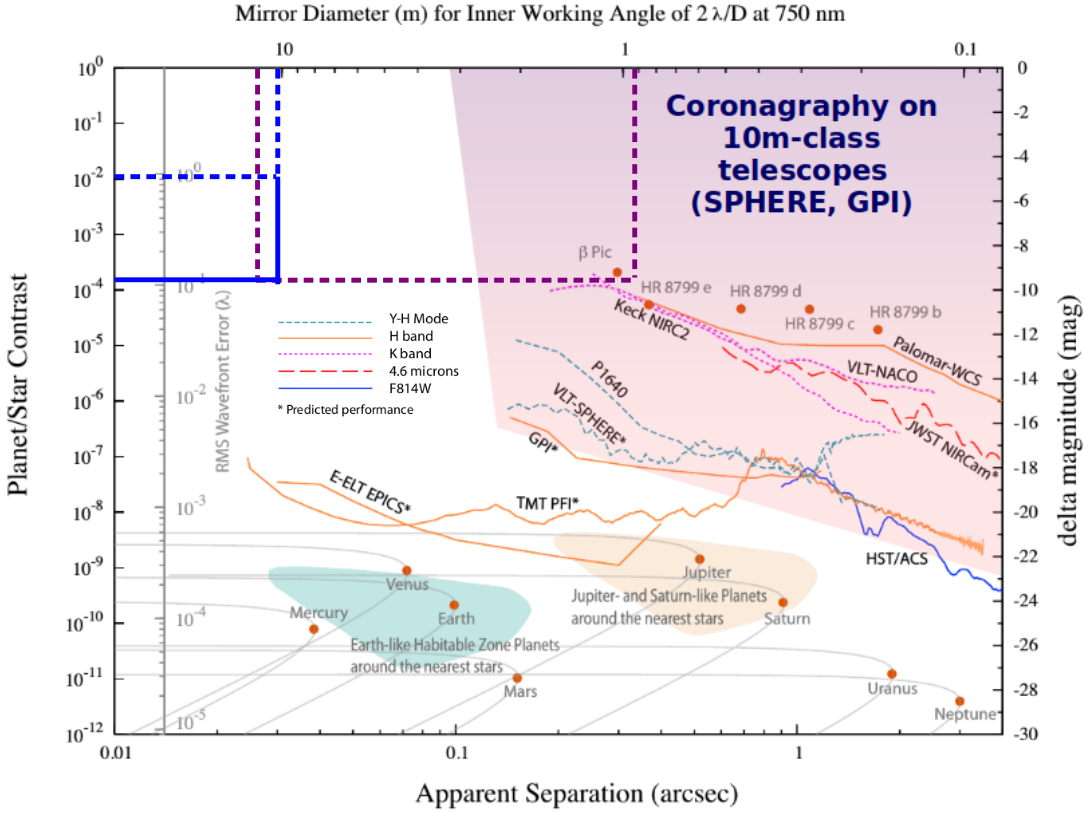
\includegraphics[width=\figwidth]{Figure_Chap1/Mawet2012_ContrastVSSeparation_InstruPerformances_02.png}
    \caption[Contraste en fonction de la séparation apparente de certaines exoplanètes imagées et des planètes du système solaire.]{Contraste (\textit{Planet/Star Contrast}) en fonction de la séparation apparente (en arcsec) des exoplanètes du système HR8799 (bcde) et de $\upbeta$ Pic b (dans la partie supérieure) et des planètes du système solaire telles que vues à une distance de $10 \,$pc (dans la partie inférieure). Un deuxième axe des ordonnées, à gauche, indique l'erreur rms (en unité de longueur d'onde) sur le front d'onde à atteindre pour imager un système exoplanétaire au contraste correspondant à la même ordonnée. Un troisième axe des ordonnées, à droite, indique la différence de magnitude entre l'étoile et la planète. Les limites hautes des performances de quelques instruments récents (Keck-NIRC2, VLT-NACO, Palomar-WCS, HST-ACS, GPI, SPHERE, Palomar-P3K-P1640 et JWST-NIRCam) et de futurs instruments (TMT-PFI et E-ELT-EPICS) sont tracées par les lignes colorées (on note que ce graphique, datant de 2012, indique par une étoile certains futurs projets qui sont actuellement en fonctionnement). Les zones verte et bleue indiquent, respectivement, les planètes de type terrestre dans la zone d'habitabilité et les planètes de type Jupiter et Saturne, autour des étoiles les plus proches. La zone de couleur violette dégradée indique le domaine de performances des systèmes coronographiques sur les télescopes de $10 \,$m. Le rectangle en tirets violets indique le domaine de performances de la technique de masquage de pupille sur les télescopes de $10 \,$m. Les rectangles en tirets bleus et en trait continu bleu indiquent les domaines de performance de la technique de masquage de pupille dans le visible des instruments FIRSTv1 et FIRSTv2, respectivement. Adapté de \cite{mawet2012}.}
    \label{fig:ContrastSeparation}
\end{figure}

Le premier défi technique à relever est le haut contraste qui est défini comme le rapport entre l'intensité lumineuse de la planète par celle de l'étoile. Celui-ci atteint $\sim 10^{-3}$ dans le cas des planètes géantes gazeuses qui émettent un rayonnement thermique infrarouge. Ce sont la plupart des systèmes imagés actuellement (ce sont les plus faciles à détecter) mais sont une population restreinte dans la taxonomie des exoplanètes car ce sont des systèmes très jeunes (de l'ordre de la dizaine de millions d'années ou moins). En revanche, le contraste des planètes de type terrestre est de $\sim 10^{-10}$. Ce sont des systèmes plus vieux (de l'ordre de centaines de millions à plusieurs milliards d'années) dans lesquels le compagnon réfléchit la lumière de l'étoile dans le visible et constituent donc un plus grand intérêt dans le cadre de la recherche de traces de vie extra-terrestre. Les systèmes imagés jusque maintenant appartiennent uniquement à la première catégorie.

La technique de la coronographie \citep{lyot1939} a été la plus largement utilisée pour obtenir ces images et son domaine de performance est représenté en dégradé de violet sur la figure~\ref{fig:ContrastSeparation}. Le composant principal de cette technique est un coronographe et il permet de supprimer (par masquage opaque ou par interférence destructive) la lumière incidente de l'étoile centrée sur son axe optique, tout en laissant apparaître la lumière du compagnon décentré par rapport à l'étoile. En revanche, les perturbations atmosphériques qui affectent le front d'onde incident lors d'observations au sol diminuent fortement les performances de cette technique. Sur la même figure, un deuxième axe vertical à gauche indique l'erreur rms maximum du front d'onde afin d'obtenir la performance en contraste correspondante. Il s'agit d'erreurs de l'ordre de $100 \,$nm rms et de $0,01 \,$nm rms dans les gammes de longueur d'onde infrarouge et visible, respectivement. Il est donc nécessaire de corriger les perturbations atmosphériques en amont du coronographe \citep{sivaramakrishnan2001} à l'aide de systèmes d'optique adaptative \citep{rousset1990} et d'optique adaptative extrême, qui permettent d'atteindre aujourd'hui des contrastes en entrée de l'instrument de $10^{-3}$ à $10^{-4,5}$ : e.g. \ac{LBTAO} \citep{esposito2011}, PALM-3000 sur le télescope Hale de l'observatoire Palomar \citep{dekany2013}, \ac{GPI} sur le télescope Gemini-South \citep{macintosh2014}, \ac{SPHERE} \citep{beuzit2019} sur le \ac{VLT}, \ac{SCExAO} \citep{jovanovic2015} sur le télescope Subaru, \ac{MagAO-X} \citep{males2020} sur le télescope Clay de l'observatoire Magellan.

Le deuxième défi est d'atteindre un fort pouvoir de résolution angulaire car il s'agit ici de détecter la lumière d'un point se trouvant à de très petites distances apparentes par rapport à l'étoile : de l'ordre de $10 - 100 \,$mas, ce qui correspond à $\sim 1 \,$ua à une distance de la Terre de $100 - 10 \,$pc. Or la coronographie n'est performante que pour des grandes séparations angulaires, typiquement égales à plus de $4 \uplambda / \text{D}$ de l'étoile centrale (avec $\uplambda$ la longueur d'onde d'observation et D le diamètre du miroir primaire du télescope) car la lumière de l'étoile parvient à fuir aux petites séparations ce qui rend difficile la détection de compagnons trop proches. De nouveaux concepts voient le jour pour améliorer cette performance des coronographes \citep{mawet2012} mais ils parviennent encore difficilement à des séparations de l'ordre de la limite de diffraction $\uplambda / \text{D}$. Le masquage de pupille (voir la section~\ref{sec:PupilMasking}) est une technique permettant d'augmenter le pouvoir de résolution en imagerie jusqu'à $0,5 \uplambda / \text{D}$. Son domaine de performance est tracé sur la figure~\ref{fig:ContrastSeparation} par les rectangles en tirets violets, en tirets bleus et en trait continu bleu, respectivement sur des télescopes de $8 - 10 \,$m dans l'infrarouge, sur \acrshort{FIRSTv1} dans le visible et \ac{FIRSTv2} dans le visible. On note l'intérêt d'observations dans le visible qui permettent de meilleures résolutions angulaires mais aussi les bas contrastes jusqu'alors atteints ($< 10^{-4}$) par cette technique dus à sa nature peu sensible. Comme nous le verrons par la suite, la technique de réarrangement de pupille est une technique permettant d'utiliser un masquage redondant de la pupille afin de contrebalancer ce problème.

Enfin, des programmes de traitement et d'analyse de données élaborés permettent d'augmenter un peu plus les performances en contraste sur les images de $1-2$ ordres de grandeur : e.g. \ac{ADI} \citep{marois2006}, \ac{SDI} \citep{marois2000}, \ac{RDI} \citep{lafreniere2009}. C'est en combinant toutes ces applications instrumentales (optique adaptative, coronographie et traitement de données approfondis) qu'il a été possible d'imager directement quelques systèmes exoplanétaires. Cela a permis d'ouvrir un nouveau domaine de l'étude des exoplanètes qui grandit toujours actuellement et qui a encore beaucoup à faire. Parmi les différentes voies existantes, l'interférométrie est une technique proposant d'atteindre de meilleures performances en résolution angulaire de plusieurs ordres de grandeur et c'est dans ce cadre que s'inscrit mon travail de thèse.


%%%%%%%%%%%%%%%%%%%%%%%%%%%%%%%%
\section{L'instrument FIRST dans le contexte de l'imagerie directe des exoplanètes}

%%%%%%%%%%%%%%%%
\subsection{L'interférométrie}

En reprenant les explications présentées dans la section 1.2.1 de la thèse d'Elsa Huby \citep{huby2013these}, chaque paire de points du front d'onde incident sur un télescope interfère et produit un interférogramme dans le plan focal. Ainsi, la tâche de diffraction dans le plan focal du télescope peut s'interpréter comme la superposition de l'ensemble de ces interférogrammes. Pour un front d'onde provenant d'une source lumineuse astrophysique (à l'infini) non résolue incident sur un télescope avec une pupille d'entrée circulaire, de diamètre D, la tâche de diffraction dans le plan focal est une fonction d'Airy, dont l'expression s'écrit :

\begin{equation}
    \text{I}_{\text{Airy}}(x) = \left( \frac{2 \text{J}_{1} (\uppi \text{D}x / \uplambda \text{f})}{\uppi \text{D}x / \uplambda \text{f}} \right)^2
\end{equation}

\noindent où f est la distance focale du télescope et $\text{J}_{1}$ est la fonction de Bessel de première espèce d'ordre 1.

Le pouvoir de résolution du télescope est défini par la largeur à mi-hauteur de cette tâche de diffraction, qui s'approxime à : $\uplambda / \text{D}$. Cela correspond au plus petit détail discernable par un télescope. De la même manière, la recombinaison interférométrique des deux faisceaux collectés à la sortie de deux télescopes séparés d'une distance B, appelée base, qui observent simultanément une source lumineuse donne un interférogramme équivalent à celui résultant de l'interférence de deux points séparés d'une distance B sur la pupille d'un télescope. Ainsi, la recombinaison de ces deux faisceaux permet l'observation d'une cible astrophysique avec un pouvoir de résolution égal à $\uplambda / \text{B}$ qui peut être augmenté en éloignant les télescopes, évitant ainsi la construction d'un télescope monolithique de diamètre égal à B.

C'est ce principe qui est implémenté actuellement dans les observatoires \ac{CHARA} \citep{tenbrummelaar2005} sur le Mont Wilson, qui peut combiner six télescopes de $1 \,$m de diamètre, avec des bases de $330 \,$m de longueur, dans le visible et l'infrarouge et \ac{VLTI} \citep{haguenauer2012} sur le Cerro Paranal, qui peut combiner quatre télescopes de $\sim 8 \,$m et quatre télescopes de $1,8 \,$m de diamètre, avec des bases de $130 \,$m de longueur, dans l'infrarouge proche et moyen. C'est sur un principe interférométrique similaire que la première image de l'environnement proche du trou noir du centre de la galaxie M87 a été construite \citep{EHTC2019}. Il s'agit dans ce cas-là d'interférométrie hétérodyne, à partir de la combinaison des faisceaux radio de télescopes répartis sur Terre, offrant une base de longueur de son diamètre ($\sim 10^4 \,$km). Mais encore, le futur projet \textit{hypertélescope} \citep{labeyrie2013} a pour ambition de combiner les faisceaux de télescopes espacés jusqu'à $10^5 \,$km dans l'espace pour l'étude des galaxies, l'étude de surfaces stellaires et l'imagerie directe d'exoplanètes.

Ces solutions techniques font partie du domaine de l'interférométrie longue base. La technique que je vais maintenant exposer et qui est implémentée dans le concept de \ac{FIRST} est l'interférométrie à masquage de pupille qui s'utilise sur un unique télescope.


%%%%%%%%%%%%%%%%
\subsection{Les techniques de masquage et réarrangement de pupille}
\label{sec:PupilMasking}

Comme nous l'avons vu dans la partie précédente, la figure mesurée dans le plan focal d'un télescope est la superposition d'une infinité d'interférogrammes. Ainsi, une infinité de paires de points de base égale à $\vv{\text{B}}$ (repéré dans le plan pupille) contribuent à une infinité d'interférogrammes de fréquence spatiale égale à $\vv{\text{B}} / \uplambda$ (avec $\uplambda$ la longueur d'onde d'observation) qui se superposent lorsqu'ils sont imagés. Dans le cas où le front d'onde incident est perturbé par la turbulence atmosphérique, y compris après la correction par un système d'optique adaptative qui laisse des résidus, ces paires de points sont déphasés et les interférogrammes (de même fréquence spatiale) ne se superposent plus. Ces perturbations brouillent les franges ce qui induit une diminution du pouvoir de résolution de l'instrument. 

La technique de masquage de pupille \citep{baldwin1986, haniff1987} propose d'appliquer un masque comportant des trous sur la pupille du télescope afin de sélectionner des paires de sous-pupilles disposées de façon non-redondante. La non-redondance assure une unique contribution de la part des paires de sous-pupilles à chaque interférogramme ce qui empêche le brouillage des franges. Cela a, par exemple, été implémenté sur l'un des télescopes Keck \citep{tuthill2000}. La figure~\ref{fig:KeckPupilMaskingA} présente le masque utilisé, disposant de $21$ trous, superposé au miroir primaire. La figure~\ref{fig:KeckPupilMaskingB} est une image du détecteur obtenue lors d'une observation avec le masque installé. La tâche est la superposition de $21 \times 20 / 2 = 210$ réseaux de franges. Enfin, la figure~\ref{fig:KeckPupilMaskingC} est la transformée de Fourier de l'image précédente, que l'on nomme plan UV des fréquences spatiales. On remarque que ce plan est échantillonné et donne l'information sur $210$ fréquences spatiales indépendantes.

\begin{figure}[ht!]
    \centering
    \begin{subfigure}[t]{0.31\textwidth}
        \centering
        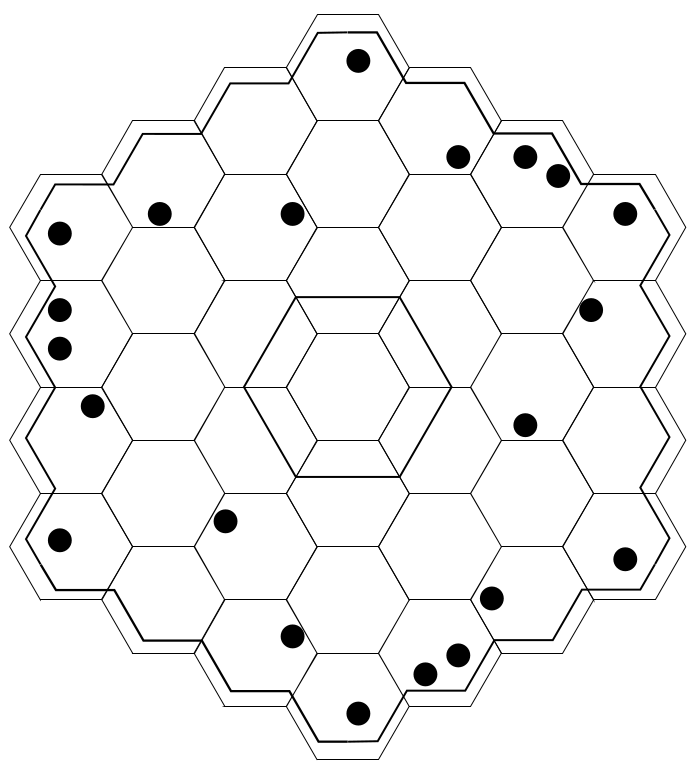
\includegraphics[width=0.9\textwidth]{Figure_Chap1/Tuthill2000_Figure3a.png}
        \caption{Pupille du télescope avec le masque. Le miroir du télescope est composé d'un pavage de segments hexagonaux et les trous du masque sont représentés par des points noirs.}
        \label{fig:KeckPupilMaskingA}
    \end{subfigure}\hspace{0.01\textwidth}
    \begin{subfigure}[t]{0.31\textwidth}
        \centering
        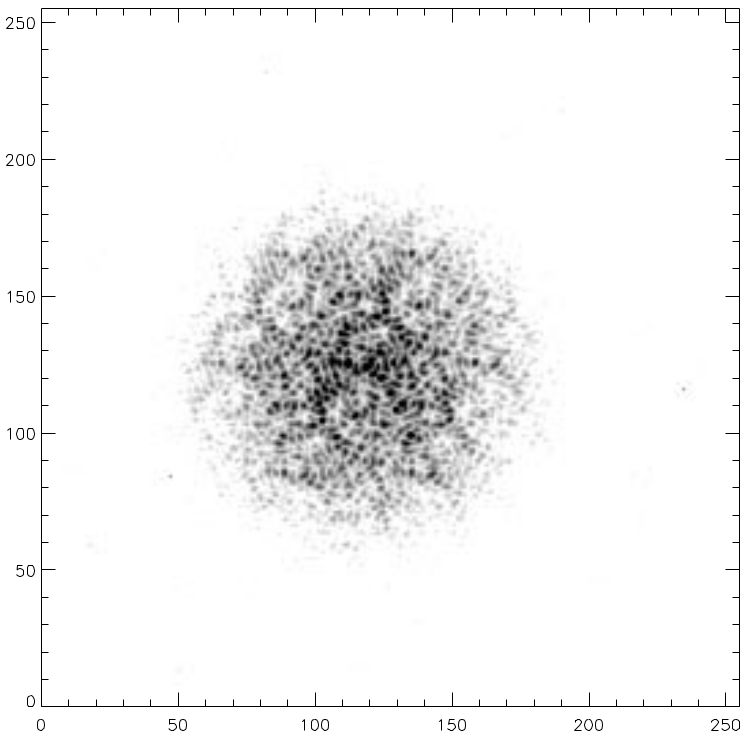
\includegraphics[width=0.9\textwidth]{Figure_Chap1/Tuthill2000_Figure3b.png}
        \caption{Image des réseaux de franges obtenus sur la caméra.}
        \label{fig:KeckPupilMaskingB}
    \end{subfigure}\hspace{0.01\textwidth}
    \begin{subfigure}[t]{0.31\textwidth}
        \centering
        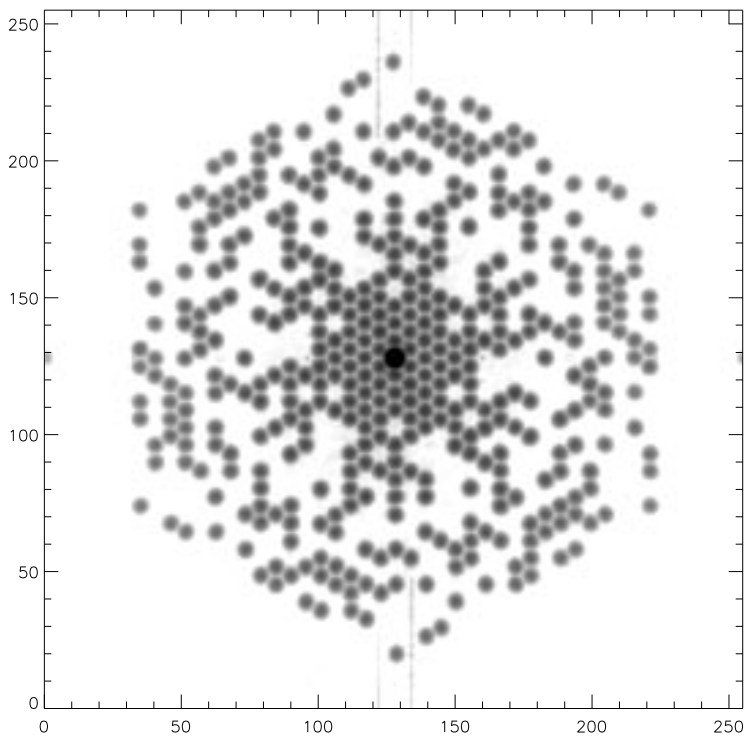
\includegraphics[width=0.9\textwidth]{Figure_Chap1/Tuthill2000_Figure3c.png}
        \caption{Plan UV obtenu par la transformé de Fourier de l'image de la caméra.}
        \label{fig:KeckPupilMaskingC}
    \end{subfigure}
    \caption[Expérience de masquage de pupille sur l'un des télescope Keck.]{Expérience de masquage de pupille sur l'un des télescope Keck. Figures tirées de \cite{tuthill2000}.}
    \label{fig:KeckPupilMasking}
\end{figure}

Cette technique a été utilisée comme mode d'observation \ac{SAM} sur l'instrument \ac{NACO} \citep{tuthill2010, lacour2011a} du \ac{VLT}, actuellement sur l'instrument \ac{SPHERE} \citep{cheetham2016} du même télescope et sur l'instrument \ac{VAMPIRES} \citep{norris2015} du télescope Subaru, ainsi que sur l'instrument \ac{NIRISS} du télescope spatial \ac{JWST} \citep{sivaramakrishnan2012}. Ce mode est aussi prévu pour l'instrument \ac{MICADO} \citep{lacour2014} du futur télescope \ac{ELT} de $39 \,$m de diamètre.

L'avantage majeur de cette technique est qu'il est possible d'atteindre, après analyse des données, un pouvoir de résolution allant jusqu'à $0,5 \uplambda / \text{D}$ où D étant le diamètre du télescope \citep{lacour2011b}. En revanche son désavantage est sa faible transmission du flux lumineux à cause de l'exploitation partielle de la pupille d'entrée du télescope. Par exemple, le masque de la figure~\ref{fig:KeckPupilMaskingA} a une transmission du flux lumineux de $10\%$.

Afin de contrebalancer ce problème, le réarrangement de pupille est proposé \citep{perrin2006, lacour2007}. Il permet d'exploiter l'entièreté de la pupille du télescope en combinaison avec la technique de masquage de pupille. Pour cela, toute la pupille est divisée en sous-pupilles afin d'être réarrangées de manière non-redondante. Pour ce faire, le flux lumineux des faisceaux de chaque sous-pupille est injecté dans des fibres optiques monomodes. Celles-ci permettent à la fois le réarrangement simple des sous-pupilles et le filtrage du front d'onde de chaque sous-pupille des résidus de phase subsistant après l'optique adaptative. \ac{FIRST} est le premier instrument implémentant cette technique de réarrangement de pupille fibré \citep{kotani2008} pour l'imagerie haut contraste à haute résolution angulaire.

Enfin, l'instrument \ac{GLINT} \citep{martinod2021}, successeur de l'instrument Dragonfly \citep{jovanovic2012}, propose une autre solution technique du réarrangement de pupille, sans fibre optique, en injectant directement les faisceaux dans un composant d'optique intégrée (servant à la recombinaison interférométrique). Les entrées ont alors la même disposition spatiale que celle des sous-pupilles. Les faisceaux sont ensuite guidés dans le composant avant d'être recombinés par paire.

Comme on vient de le voir, ces techniques atteignent un pouvoir de résolution allant jusqu'à $0,5 \uplambda / \text{D}$. Le masquage de pupille sur un télescope unique de $8 \,$m de diamètre permet des mesures sur un compagnon d'étoile avec une séparation de l'ordre de la dizaine de mas. De plus, l'étude faite par \cite{fernandes2019} sur la population des planètes géantes ($0,1 - 20 \text{M}_{\text{J}}$) détectées par la méthode des vitesses radiales et par la mission Kepler, résumée par le graphique de la figure~\ref{fig:Fernandes2019F2}, montre une forte occurrence des exoplanètes avec un demi-grand axe égal à $\sim 2 \,$ua. Or pour des systèmes exoplanétaires à une distance d'environ $100 \,$pc de la Terre (la distance où se trouve le regroupement d'étoiles en formation le plus proche), de telles valeurs de demi-grand axe, représentent une séparation projetée sur le ciel qui vaut $\sim 20 \,$mas.

\begin{figure}[ht!]
    \centering
    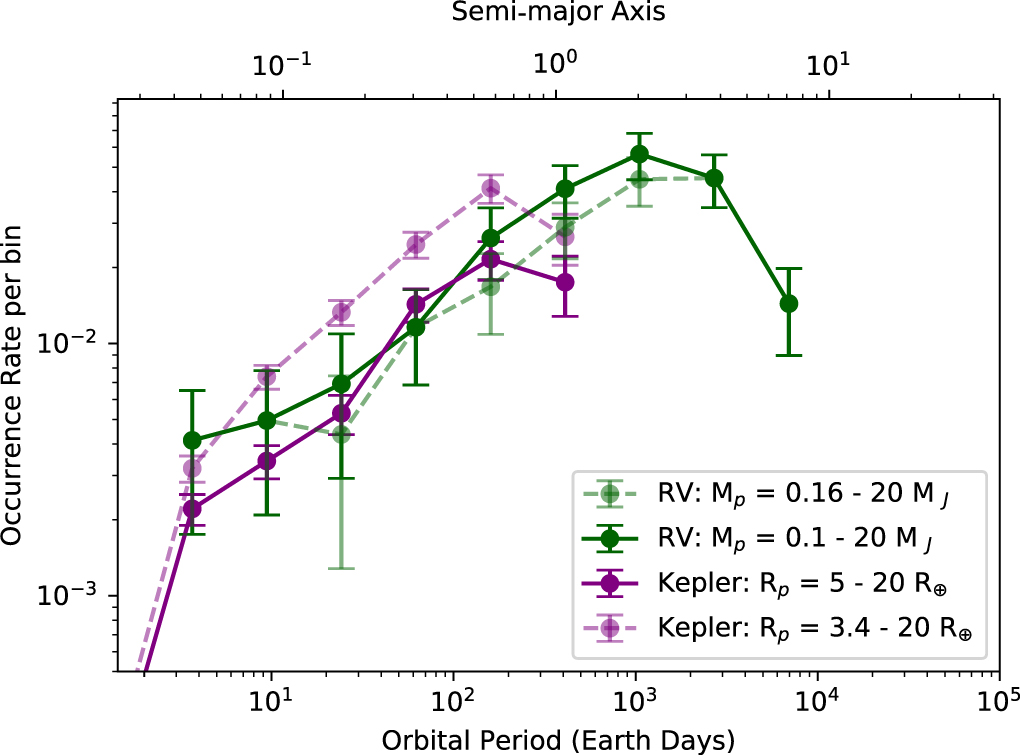
\includegraphics[width=\figwidth]{Figure_Chap1/Fernandes2019_Figure02.jpg}
    \caption[Le nombre d'occurrence des exoplanètes détectées par la méthode des vitesses radiales et par la mission Kepler en fonction de la période orbitale et du demi-grand axe.]{Le nombre d'occurrence des exoplanètes géantes en fonction de la période orbitale (axe du bas) et du demi-grand axe (axe du haut) détectées par la méthode des vitesses radiales (ligne continue verte) et par la mission Kepler (ligne continue violette). Les courbes sont données pour plusieurs intervalles de masse et de rayon (lignes continues ou discontinues). Figure tirée de \cite{fernandes2019}.}
    \label{fig:Fernandes2019F2}
\end{figure}

L'utilisation de cette technique a déjà fait certaines découvertes de compagnon sub-stellaires. Par exemple, le mode \ac{SAM} de l'instrument \ac{NACO} du \ac{VLT} a permis la découverte d'un compagnon autour de l'étoile HD 142527 \citep{biller2012} avec une séparation de $\sim 88 \,$mas, correspondant à un demi-grand axe estimé à $\sim 13 \,$ua. Le compagnon a ensuite été observé et confirmé en \ha~\citep{close2014} et son taux d'accrétion a été estimé. Cette détection ont été effectuée en infrarouge et le développement de la technique de masquage et réarrangement de pupille dans la gamme des longueurs d'onde du visible, sur des télescopes de la classe $10 \,$m de diamètre, permettrait d'augmenter encore les performances en résolution angulaire tout en permettant la caractérisation d'exoplanètes en formation (voir la section~\ref{sec:Protoplanetes}).


%%%%%%%%%%%%%%%%
\subsection{De FIRSTv1 à FIRSTv2}

L'instrument \ac{FIRST} a été développé \citep{kotani2008} pour appliquer le masquage et le réarrangement de pupille fibré combiné avec un spectrographe, dans la gamme de longueurs d'onde du visible, selon le concept développé par Sylvestre Lacour pendant sa thèse \citep{lacour2010} à partir de l'idée proposée par Guy Perrin \citep{perrin2006}. La figure~\ref{fig:FIRSTv1Scheme} présente un schéma de principe de cet instrument. La pupille du télescope est divisée en sous-pupilles représentée par le miroir déformable segmenté (1) dont les segments bleus (au nombre de $9$) sont ceux dont la lumière est injectée dans les fibres optiques monomodes (3) à l'aide d'une matrice de micro-lentille (2). Les fibres sont connectées aux fibres d'un V-Groove (la figure~\ref{fig:VGroove} présente des photographies de ce composant) de manière non-redondantes (4) où les sorties sont disposées sur une dimension (réarrangement de pupille). Les sorties du V-Groove sont dispersées par un spectrographe (5) et imagées sur la caméra dont une image est montrée (6). Ici les longueurs des fibres optiques ont dû être égalisées afin d'annuler les retards de phase entre les faisceaux des sous-pupilles au moment d'interférer dans le plan focal (6).

\begin{figure}[ht!]
    \centering
    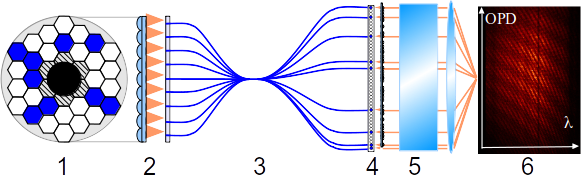
\includegraphics[width=\figwidth]{Figure_Chap1/FIRSTv1Scheme_36Outputs_Fringes_b.png}
    \caption[Schéma de principe de FIRSTv1.]{Schéma de principe de FIRSTv1. La lumière se propage de gauche à droite, sur les composants suivants : (1) le miroir segmenté représenté avec l'obstruction centrale du télescope, (2) la matrice de micro-lentilles, (3) les fibres optiques monomodes, (4) le V-Groove pour le réarrangement de pupille, (5) le spectrographe et (6) la caméra. Crédit : Elsa Huby.}
    \label{fig:FIRSTv1Scheme}
\end{figure}

L'instrument a ensuite été intégré pour sa première lumière \citep{huby2012} sur le télescope de $3 \,$m Shane de l'observatoire Lick durant la thèse d'Elsa Huby \citep{huby2013these}. La figure~\ref{fig:FIRSTv1PupilMaskingA} présente le masquage de pupille utilisé sur \ac{FIRST} (à gauche) et leur réarrangement non-redondant à $1$ dimension à l'aide d'un V-Groove (à droite). \ac{FIRST} a ainsi pu recombiner jusqu'à $18$ sous-pupilles (via deux masques sur la même pupille et deux V-Grooves). Une image des réseaux de franges mesurée lors d'une des premières observations de Véga ($\upalpha$ Lyr) est présentée sur la gauche de la figure~\ref{fig:FIRSTv1PupilMaskingB} sur laquelle l'axe vertical est l'axe des \ac{OPD}s et l'axe horizontal est l'axe des longueurs d'onde. Sur cette image on voit la superposition de $9 \times 8 / 2 = 36$ réseaux de franges donnant l'information de $36$ fréquences spatiales. Enfin, la partie droite de la figure~\ref{fig:FIRSTv1PupilMaskingB} présente la densité spectrale de puissance (obtenue par la transformée de Fourier) de l'image précédente, sur laquelle on voit les pics de fréquences spatiales échantillonnées.

\begin{figure}[ht!]
    \centering
    \begin{subfigure}[t]{0.45\textwidth}
        \centering
        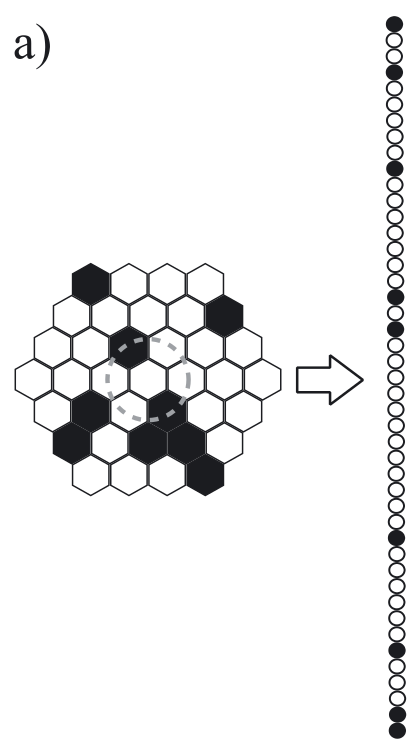
\includegraphics[width=0.7\textwidth]{Figure_Chap1/Huby2012_Figure2a.png}
        \caption{À gauche, la configuration des sous-pupilles choisies, à droite, la configuration 1-D choisie pour le réarrangement de pupille.}
        \label{fig:FIRSTv1PupilMaskingA}
    \end{subfigure}\hspace{0.01\textwidth}
    \begin{subfigure}[t]{0.45\textwidth}
        \centering
        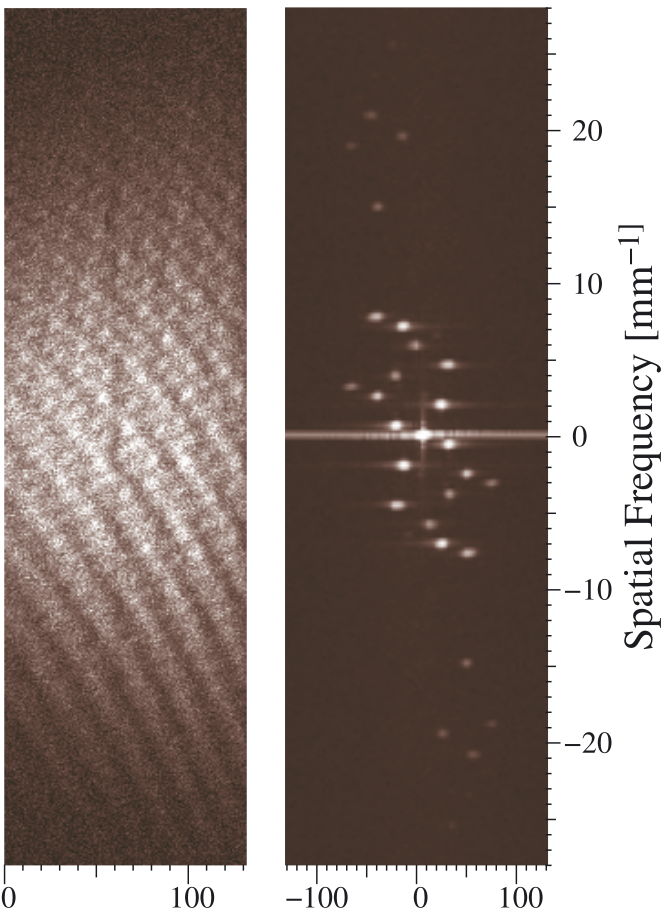
\includegraphics[width=0.9\textwidth]{Figure_Chap1/Huby2012_Figure3.png}
        \caption{À gauche, une image des réseaux de franges mesurée sur la caméra lors d'une observation de Véga à l'observatoire Lick, à droite la densité spectrale de puissance de cette image, montrant la répartition de l'échantillonnage du plan UV.}
        \label{fig:FIRSTv1PupilMaskingB}
    \end{subfigure}
    \caption[Expérience de réarrangement de pupille de l'instrument FIRSTv1 sur le télescope Shane.]{Expérience de masquage et de réarrangement de pupille de l'instrument FIRSTv1 sur le télescope Shane, tiré de \cite{huby2012}.}
    \label{fig:FIRSTv1PupilMasking}
\end{figure}

De cette manière, les performances de ces techniques ont été démontrées durant la thèse d'Elsa Huby \citep{huby2013} à partir d'observations sur l'étoile multiple Capella ($\upalpha$ Aur) sur le télescope de $3 \,$m Shane de l'observatoire Lick. La séparation des deux composantes résolues par \ac{FIRST} est estimée à $50 \,$mas avec une précision de l'ordre de $1 \,$mas, ce qui est en-deçà du pouvoir de résolution du télescope ($58 \,$mas à $850 \,$nm). Les positions mesurées d'une des deux composantes (l'autre étant centrée dans le champ de vue du télescope) ont été trouvées en accord avec l'orbite connue. Cela a aussi donné lieu à la première mesure du spectre du rapport de flux des deux composantes ($\sim 1$) aux longueurs d'onde $600 - 850 \,$nm avec une résolution spectrale de $\sim 300$. Des raies d'émission ont pu être identifiées (notamment la raie \ha, les bandes TiO et CN) et analysées en regard de simulations.

À la fin de sa thèse, Elsa Huby a mené l'intégration de \ac{FIRST} sur la plateforme \ac{SCExAO} sur le télescope de $8 \,$m Subaru. Le concept est resté le même et cela a permis de bénéficier du plus grand miroir du Subaru afin d'augmenter le flux lumineux injecté dans l'instrument ainsi que son pouvoir de résolution, tout en bénéficiant de la correction extrême d'optique adaptative de la plateforme \ac{SCExAO} ainsi que la meilleure qualité de ciel (en terme de turbulence atmosphérique) à disposition sur Terre, qu'offre le site d'Hawaii. Cela permet en conséquence d'acquérir des images interférométriques avec un temps d'exposition plus long et donc d'augmenter la sensibilité de l'instrument. Les premiers résultats et la démonstration de l'instrument sur ciel ont été publiés par Sébastien Vievard dans \cite{vievard2020a} et Vievard et al. (2023, en préparation) afin de démontrer la faisabilité du concept sur un télescope faisant partie de la classe des télescopes d'une dizaine de mètres de diamètre avec un système d'optique adaptative extrême, grâce à de nouvelles observations sur le système Capella ($\upalpha$ Aur). La figure~\ref{fig:FIRSTv1PupilMaskingSubaru} présente le masquage de pupille sur \ac{FIRST}, sur le télescope Subaru \citep{vievard2020a}. Comme la figure précédente, à gauche est la configuration des sous-pupilles choisies (les deux couleurs indiquent les deux groupes de neuf sous-pupilles injectés dans les deux bras de \ac{FIRST}), au milieu est une image des sorties photométriques d'un des deux V-Grooves ce qui montre la configuration 1-D du réarrangement de pupille et à droite est une image des réseaux de frange sur la source interne.

\begin{figure}[ht!]
    \centering
    \begin{subfigure}[t]{0.49\textwidth}
        \centering
        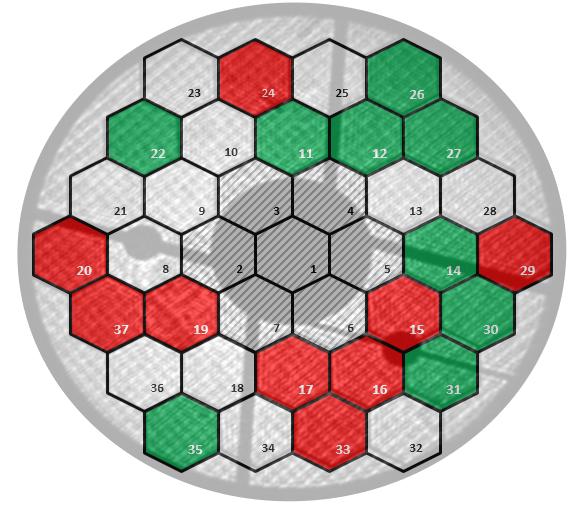
\includegraphics[width=\textwidth]{Figure_Chap1/Vievard2020_Figure5.png}
        \caption{À gauche, la configuration des sous-pupilles choisies, superposée au plan pupille d'entrée de FIRST. Deux jeux de neuf fibres permettent l'injection et la recombinaison des deux groupes de sous-pupilles, en vert en rouge.}
        \label{fig:FIRSTv1PupilMaskingSubaruA}
    \end{subfigure}\hspace{0.01\textwidth}
    \begin{subfigure}[t]{0.49\textwidth}
        \centering
        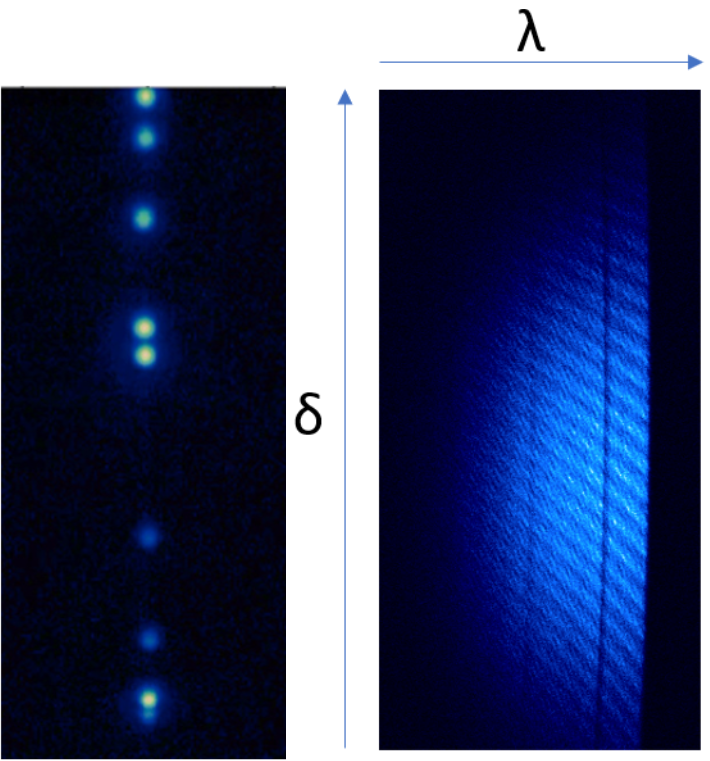
\includegraphics[width=0.9\textwidth]{Figure_Chap1/Vievard2020_Figure4.png}
        \caption{À gauche, une image des sorties photométriques des neuf fibres d'un des deux V-Grooves, montrant la configuration 1-D du réarrangement de pupille. À droite, une image des réseaux de franges mesurée sur la caméra sur la source interne, avec la dispersion sur l'axe horizontal et l'opd sur l'axe vertical.}
        \label{fig:FIRSTv1PupilMaskingSubaruB}
    \end{subfigure}
    \caption[Expérience de réarrangement de pupille de l'instrument FIRSTv1 sur le télescope Subaru.]{Expérience de masquage et de réarrangement de pupille de l'instrument FIRSTv1 sur le télescope Subaru, tiré de \cite{vievard2020a}.}
    \label{fig:FIRSTv1PupilMaskingSubaru}
\end{figure}

Une réplique de cet instrument a été développée par Nick Cvetojevic sur le banc de test \ac{FIRSTv2} au laboratoire \ac{LESIA} (à Meudon) dans le but de tester de nouvelles solutions de recombinaison des sous-pupilles. Ce banc de test est amplement détaillé dans la section~\ref{sec:FIRSTv2Concept} mais je résume son principe ici. Il s'agit de recombiner indépendamment les faisceaux par paire en injectant les faisceaux des sous-pupilles dans un composant d'optique intégrée, là où sur la première version les faisceaux interféraient dans le plan focal de l'instrument. Cette technologie est dite photonique car elle consiste en un bloc de verre dans lequel sont gravés des guides d'onde. Les faisceaux des n sous-pupilles y sont injectés, puis sont divisés en $\text{n} - 1$ sous-faisceaux pour être ensuite recombinés par paire. Enfin, les sorties de la puce sont connectées aux fibres d'un V-Groove, dont ses sorties (qui n'ont pas besoin d'être disposées de manière non-redondante comme précédemment) sont dispersées par un spectrographe et imagées sur un détecteur. La figure~\ref{fig:FIRSTv2FringesCameraB} présente les interférogrammes obtenus sur ce banc de test imagés par la caméra, pour la configuration de sous-pupilles montrée sur la figure~\ref{fig:FIRSTv2FringesCameraA} (pour plus de détails voir la section~\ref{sec:BaseConfig}). Chaque interférogramme est imagé sur des pixels différents sur le détecteur selon l'axe vertical, en étant dispersés selon l'axe horizontal. On note que ces interférogrammes sont pour une valeur d'\ac{OPD} et les franges sont mesurées sur l'axe des \ac{OPD}s grâce au miroir segmenté qui est contrôlable en piston. L'objectif avec cette nouvelle version est d'augmenter les performances en contraste et en sensibilité afin de permettre des mesures de systèmes exoplanétaires présentant de plus hauts contrastes.

\begin{figure}[ht!]
    \centering
    \begin{subfigure}[t]{0.4\textwidth}
        \centering
        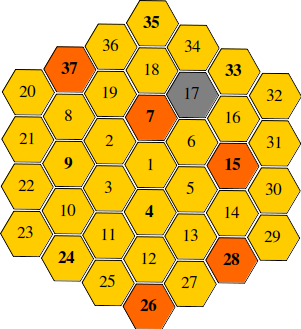
\includegraphics[width=0.9\textwidth]{Figure_Chap2/BaselineMap_Meudon_37_7_26_15_28.png}
        \caption{Configuration des sous-pupilles choisies sur FIRSTv2.}
        \label{fig:FIRSTv2FringesCameraA}
    \end{subfigure}
    \begin{subfigure}[t]{0.55\textwidth}
        \centering
        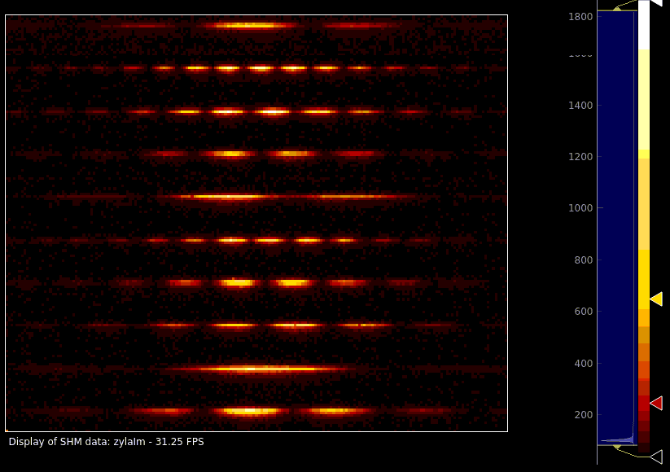
\includegraphics[width=0.9\textwidth]{Figure_Chap1/20220505_5TC_AY_InjectionOpti_Fringes_Meudon_crop.png}
        \caption{Image des interférogrammes sur la fenêtre de visionnage temps réel de la caméra de FIRSTv2 sur une source interne.}
        \label{fig:FIRSTv2FringesCameraB}
    \end{subfigure}
    \caption[Expérience de réarrangement de pupille de l'instrument FIRSTv2.]{Expérience de masquage et réarrangement de pupille de l'instrument FIRSTv2.}
    \label{fig:FIRSTv2PupilMasking}
\end{figure}

L'instrument \ac{GRAVITY} implémente une puce photonique \citep{perraut2018} dans le proche infrarouge qui recombine les faisceaux des quatre télescopes du \ac{VLT}. Cela a mené à la première détection directe d'une exoplanète par interférométrie \citep{lacour2019} ce qui démontre la capacité de cette technologie pour l'étude de systèmes exoplanétaires. Le développement de \ac{FIRSTv2} se fait dans les gammes de longueurs d'onde du visible afin d'améliorer les performances en résolution angulaire des mesures (celle-ci étant proportionnelle à la longueur d'onde) et de permettre la détection de la raie \ha~dans le spectre de protoplanètes, qui est probablement crucial pour la caractérisation des systèmes protoplanétaires, comme nous le verrons plus loin (section~\ref{sec:AccretionAlpha}).

Pour finir, \ac{FIRST} permet d'évaluer les futures performances de l'ensemble des techniques que nous avons vues ici sur les futurs \ac{ELT} de $> 30 \,$m de diamètre \citep{vievard2020b}. Un tel concept d'instrument sur cette classe de télescopes permettrait d'atteindre un pouvoir de résolution angulaire égal à $\sim 2 \,$mas à $700 \,$nm, sur des systèmes avec un contraste allant jusqu'à $10 ^{-6}$. Cela augmenterait le nombre de candidats d'exoplanètes au champ de l'imagerie directe mais aussi à d'autres domaines d'études comme les centres actifs des galaxies dans le visible.


%%%%%%%%%%%%%%%%
\subsection{L'apport de ma thèse au projet FIRST}

Le travail de ma thèse s'inscrit dans la continuité du développement de la réplique de \ac{FIRST} au laboratoire à Meudon. L'objectif est de tester en laboratoire la technologie d'optique intégrée pour la recombinaison interférométrique des sous-pupilles. Cette technologie dans les gammes de longueur d'onde du visible est nouvelle dans le domaine de l'astronomie. En effet, elle a été développée et optimisée ces dernières décennies dans le domaine des télécommunications en infrarouge et son adaptation dans le domaine du visible nécessite de nombreuses années de développement et de test. J'ai ainsi caractérisé deux technologies différentes de composants d'optique intégrée, présentés dans la section~\ref{sec:FIRSTv2Concept}, dans laquelle je présente toute l'expérience \ac{FIRSTv2}. 

De plus, une partie de mon travail de thèse a été de développer le logiciel de contrôle afin de le restructurer pour l'améliorer et d'ajouter de nouvelles fonctionnalités. Je présenterai ce travail dans la section~\ref{sec:ControlSoftware}. Ensuite, j'ai travaillé sur le développement du programme de traitement et d'analyse de données (section~\ref{sec:DataReduction}). Ce programme permet d'analyser des données acquises sur une source de type protoplanétaire que j'exposerai dans la section~\ref{sec:Protoplanetes}. J'ai alors démontré pendant ma thèse, la capacité de l'instrument \ac{FIRSTv2} à détecter une telle cible en intégrant au banc de test un système de sources lumineuses simulant une protoplanète compagnon d'une étoile (section~\ref{sec:SystBinaire}), en acquérant des données interférométriques sur celle-ci et en les traitant avec le programme développé pour l'occasion. Il s'agissait également d'implémenter pour la première fois sur le projet \ac{FIRST} la mesure des phases différentielles, qui est une observable particulièrement bien adaptée à la détection de systèmes protoplanétaires. Je présenterai les résultats de ces mesures dans la section~\ref{sec:BinaryCharac}. 

Enfin, la dernière partie de ma thèse a été l'intégration des puces photoniques sur la plateforme \ac{SCExAO} au télescope Subaru, pour la prise de données sur ciel lors de la première lumière de \ac{FIRSTv2}, que je présenterai dans la section~\ref{sec:FIRSTv2Subaru}. Lors de cette première lumière j'ai aussi eu l'occasion de déployer le logiciel de contrôle que j'avais développé et testé en laboratoire, à Meudon.


%%%%%%%%%%%%%%%%%%%%%%%%%%%%%%%%
\section{L'observation des systèmes protoplanétaires}
\label{sec:Protoplanetes}

%%%%%%%%%%%%%%%%
\subsection{La formation planétaire}

La variété des exoplanètes jusqu'alors détectées permet d'étudier des conditions physiques, astrométriques et chimiques différentes, constituant une source d'informations pour la compréhension des systèmes planétaires. Notamment, l'étude de leur stade évolutif retient notre attention ici et est possible en étudiant différents systèmes d'exoplanètes se trouvant à différents stades de leur formation. 

Tout d'abord, l'étoile centrale se forme par effondrement de matière au sein d'un nuage de gaz, dominé par de l'hydrogène moléculaire. Lorsqu'un corps de quelques masses de Jupiter est formé, la densité y est suffisante pour qu'il y ait un état d'équilibre hydrostatique dans lequel la force de gravité compense la force de pression de la matière. Tout en s'effondrant sur l'étoile, le nuage de gaz acquiert un moment cinétique dominant et, en conséquence, se répartit sur un disque en rotation par effet centrifuge, ce qui explique que l'on retrouve les planètes et beaucoup de corps divers du système solaire sur un même plan (l'écliptique). Ce disque protoplanétaire \citep{williams2011} se forme rapidement, en moins de $10 \,$kyr et est à des températures telles qu'il est observable dans les grandes longueurs d'ondes millimétriques et infrarouges. La figure~\ref{fig:DiskEvo} est une schématisation des étapes majeures de l'évolution de ce disque. L'étoile est totalement formée en $0.5 - 1 \,$Myr et induit sur le disque des rayonnements \ac{UV} qui ont pour effet d'évacuer tout le gaz de la partie interne du disque vers les plus lointaines orbites en l'espace de $\sim 0.1 \,$Myr (figure~\ref{fig:DiskEvo} (a), (b) et (c)). Jusqu'à environ $10 \,$Myr, le disque est encore protoplanétaire et est optiquement épais (la lumière visible ne s'échappe pas de l'intérieur du disque). Il contient encore du gaz primordial ainsi que de la poussière mais des intervalles vides se forment déjà, dus à la présence de protoplanètes. Entre $\sim 10 \,$Myr et $\sim 100 \,$Myr le disque est appelé disque de débris \citep{wyatt2008} car il ne contient plus du tout de gaz, qui a été accrété par les planètes, et il est constitué de poussières de seconde génération, provenant des nombreuses collisions d'astéroïdes et de planétésimaux (figure~\ref{fig:DiskEvo} (d)). L'âge maximal typique d'un disque de débris est de quelques $100 \,$Myr. Il est possible d'étudier ces détails des systèmes planétaires via les mesures de leur spectre électromagnétique. En effet, selon la taille des grains de poussières (qui augmente avec le temps) le rayonnement détecté évoluera vers les courtes longueurs d'ondes. De plus, les disques protoplanétaires, dans leurs premiers stades d'évolution, sont optiquement épais et l'étude de la répartition spectrale d'énergie permet d'inférer dans quelle mesure le disque modifie le spectre de l'étoile centrale.

\begin{figure}[ht!]
    \centering
    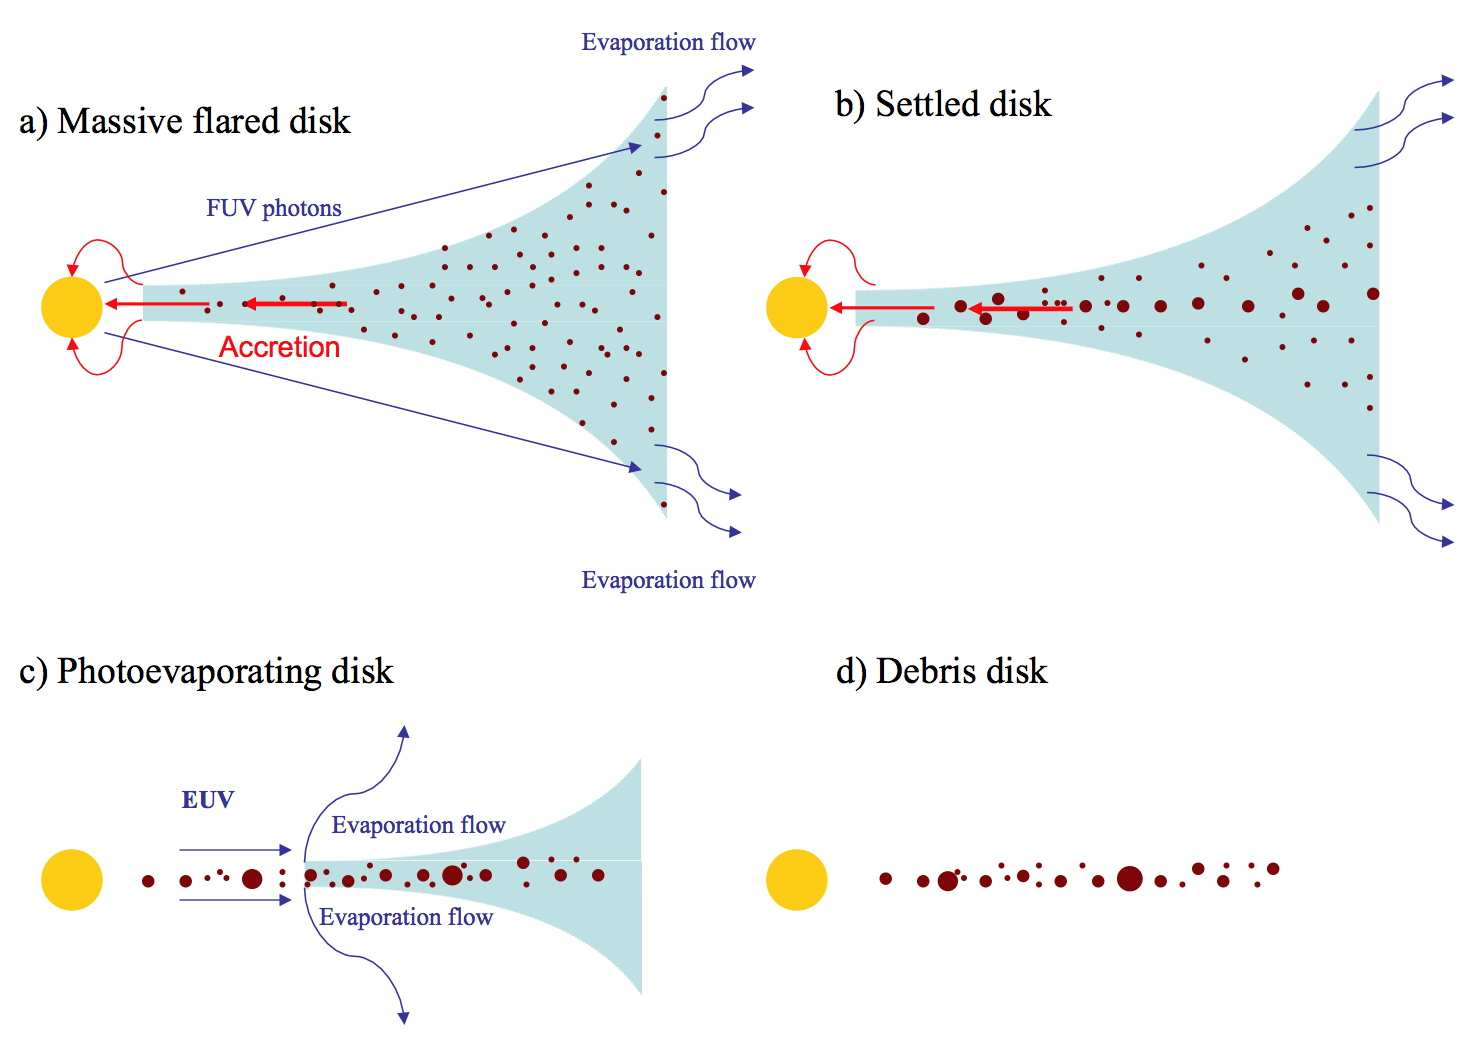
\includegraphics[width=\figwidth]{Figure_Chap1/Williams2011_Fig06_PlanetaryDiskEvolution.png}
    \caption[Évolution typique d'un disque protoplanétaire.]{Évolution typique d'un disque protoplanétaire, tiré de \cite{williams2011}. Le gaz est représenté en bleu et les poussières en marron. (a) Le disque dans son stade d'évolution primitif ($0-1\,$Myr) perd de la matière par accrétion sur l'étoile et photo-évaporation par les rayonnements \ac{UV} émis par l'étoile. (b) Les grains de poussières s'agglomèrent en débris de plus en plus gros tout en se répartissant sur un même plan. (c) L'étoile a fini de se former et le disque interne est dépourvu de gaz, devenant optiquement fin en quelques $0.1 \,$Myr. (d) Les plus petits grains de matière soit se font éjecter par pression de radiation soit sont accrétés par les planètes et il ne reste que les planétésimaux au sein du disque, qui devient de plus en plus difficile à détecter, en l'espace de quelques $100 \,$Myr.}
    \label{fig:DiskEvo}
\end{figure}

Dans le même temps, on identifie $3$ stades d'évolutions des exoplanètes observées, pendant lesquels les exoplanètes sont nommées :

\begin{enumerate}
    \item protoplanètes lorsque le système est âgé de moins de $4 \,$Myr, ce sont les exoplanètes qui m'intéressent dans le cadre de mon projet de thèse, elles sont toujours en formation et accrètent de la matière, au sein du disque protoplanétaire et ont une forte émission dans la raie \ha~(comme on le verra plus en détails dans la section~\ref{sec:AccretionAlpha});
    
    \item jeunes planètes géantes lorsque le système est âgé de $4 \,$Myr à $100 \,$Myr, elles sont au sein d'un disque de débris, elles n'accrètent plus de matière mais ont une température assez élevée ($\sim 700 - 1700 \,$K) pour émettre un rayonnement thermique visible et infrarouge et font partie du groupe d'exoplanètes les plus détectées en imagerie directe (e.g. Beta Pictoris b \citep{lagrange2010});
    
    \item planètes complètement formées lorsque le système est âgé de plus de $100 \,$Myr, constituant la grande majorité des exoplanètes connues, elles sont trop froides pour rayonner dans le visible (elles n'ont qu'un rayonnement infrarouge) comme sur les deux types d'exoplanètes précédemment cités, mais peuvent refléter suffisamment la lumière de leur étoile pour être détectées en imagerie directe (dans le visible).
\end{enumerate}

À ce jour, deux grandes théories existent pour décrire les mécanismes de formation planétaire. La première théorie est la formation par accrétion de matière (\ac{CA}, en anglais), pour la première fois énoncée dans \cite{safronov1972}. Les grains de poussières microscopiques se combinent pour former des corps de plus en plus gros : des astéroïdes, puis des planétésimaux (future planète). Enfin, si ces corps ont une masse d'au moins $10 \,$ M$_{\bigoplus}$, ils accrètent du gaz et deviennent des géantes gazeuses \citep{pollack1996}. Pour le système solaire, cela explique donc bien la présence de quatre planètes rocheuses dépourvues de gaz car il a été expulsé par le Soleil (comme expliqué dans le paragraphe précédent) sur les plus petites orbites ainsi que de planètes géantes gazeuses sur les orbites les plus lointaines et dont on soupçonne qu'elles contiennent un noyau rocheux.

Bien que cette première théorie soit la plus acceptée par la communauté, notamment pour expliquer la formation du système solaire, de récents travaux montrent qu'une deuxième théorie est plausible. Cette théorie fait appel à des processus d'instabilité gravitationnelle (\ac{GI}, en anglais) et est, par exemple, simulée dans \cite{nayakshin2017}. Ici, juste après la formation de l'étoile, des régions localisées dans le disque exoplanétaire se condensent par instabilités gravitationnelles en des corps de plusieurs fois la masse de Jupiter. Dans ces conditions, les grains de poussière sédimentent et forment un noyau rocheux central. Certaines simulations \citep{boley2010} montrent que ces amas se forment à $\gtrsim 50 \,$ua et migrent jusqu'aux basses orbites ($\sim 1 \,$ua), où ils perdent leur couche de gaz à cause des effets de marée. Cela réussit aussi à expliquer la présence de petites planètes rocheuses aux orbites les plus proches du Soleil et des géantes gazeuses dotées de noyaux rocheux sur des orbites plus éloignées, où les effets de marée ne sont pas suffisamment forts pour dissiper leur gaz.

Il est probable que les mécanismes de ces deux théories soient à l'oeuvre au cours de la formation planétaire. L'étude d'un plus grand nombre de systèmes protoplanétaires est donc indispensable pour contraindre ces théories.


%%%%%%%%%%%%%%%%
\subsection{L'accrétion de matière des protoplanètes}
\label{sec:AccretionAlpha}

Comme nous l'avons vu dans la section~\ref{sec:ImagerieDirecte}, l'imagerie directe permet l'étude de systèmes exoplanétaires encore jamais étudiés et permet une étude photométrique et spectroscopique de ceux-ci. Cette technique est adaptée à l'observation de protoplanètes car, d'une part, ce sont des systèmes jeunes et chauds donc ce sont les plus lumineux et, d'autre part, elle permet la mesure d'observables directement liées aux processus de formation planétaire.

L'une de ces observables qui nous intéresse est le spectre d'émission. En effet, l'accrétion de matière par un astre induit l'émission de raies associées à l'hydrogène dans le spectre mesuré. Lorsque le gaz, principalement composé d'hydrogène s'effondre sur une étoile ou une planète, il atteint des vitesses qui dépassent la vitesse du son locale. Le gaz génère en conséquence des ondes de choc augmentant la température de plusieurs milliers à plusieurs dizaines de milliers de Kelvins. À cette température, l'hydrogène est excité et émet les raies spectrales des bandes Lyman, Balmer, Paschen, etc. Ces émissions ont été simulées pour des proto-étoiles jeunes en accrétion à partir de modèles d'accrétion magnétosphérique \citep{muzerolle2001, natta2004, espaillat2008}, dans lesquels le gaz interagit avec le champ magnétique stellaire, permettant ainsi de déterminer les liens entre ces émissions et le taux d'accrétion. De telles émissions aux longueurs d'onde des raies de l'hydrogène ont été mesurées pour un échantillon d'étoiles jeunes du nuage Lupus \citep{alcala2014, alcala2017}, permettant d'estimer leur taux d'accrétion de matière ainsi que les liens entre la géométrie des flux d'accrétion et le taux d'accrétion. Une étude similaire sur le taux d'accrétion de l'étoile PDS 70 a aussi été conduite dans \cite{thanathibodee2020} en utilisant un modèle d'accrétion magnétosphérique. PDS 70 est dite de type T Tauri (\ac{TTS}, en anglais) \citep{appenzeller1989}, qui définit les étoiles variables jeunes en formation, de masse de moins de $2 \, \MS$, âgées de moins de $10 \,$Myr et appartenant à la pré-séquence principale (PDS 70 est de type spectral K7). Comme beaucoup d'étoiles de type \ac{TTS}, PDS 70 est dotée d'un disque de transition (stade d'évolution entre le disque protoplanétaire et le disque de débris) ainsi que d'un champ magnétique. Ces disques se caractérisent par la présence d'orbites pratiquement vides contenant parfois des protoplanètes. Les taux d'accrétion d'étoiles de type \ac{TTS} ont plusieurs fois été calculés \citep{natta2004, rigliaco2012, ingleby2013}, permettant d'éprouver les modèles et techniques de calcul de taux d'accrétion, mais de grandes incertitudes demeurent.

Ces modèles d'accrétion de matière, initialement développés pour des étoiles jeunes et peu massives, ont été adaptés pour le cas de protoplanètes \citep{aoyama2018, thanathibodee2019}. Les difficultés d'une telle adaptation sont que les conditions d'accrétion sur les protoplanètes sont différentes de celles sur les étoiles : dans le cas des protoplanètes, (1) la température du gaz en accrétion est moins élevée (d'au moins un ordre de grandeur), (2) le milieu dans le voisinage de la protoplanète (le disque circumplanétaire) n'a pas les mêmes structures (c'est parfois un bras de gaz et de poussière \citep{boccaletti2020} approvisionnant en matière l'étoile encore en formation) et (3) les champs magnétiques locaux sont différents en intensité et en structure, entraînant des écoulements de gaz différents dans l'un ou dans l'autre des cas. Plus simplement, dans le cas des étoiles de type \ac{TTS}, le gaz est excité avant le choc supersonique et est ionisé après le choc car les champs magnétiques locaux sont assez puissants pour accélérer les écoulements alors que dans le cas des protoplanètes, le gaz n'est excité seulement qu'après le choc supersonique \citep{aoyama2019}.

L'étude des raies d'émission hydrogène de Balmer, plus particulièrement la raie Balmer-$\alpha$ ($656.28 \,$nm), aussi appelée raie \ha, est un bon moyen d'estimer le taux d'accrétion de matière en cours sur les protoplanètes \citep{aoyama2019, marleau2022}. \ac{FIRSTv2} est conçu pour travailler dans cette gamme de longueur d'onde et ainsi détecter une raie \ha. C'est pour cela que, dans la suite, je vais m'intéresser essentiellement aux travaux effectués sur la détermination du taux d'accrétion à partir de la mesure de cette raie.

À partir du spectre mesuré, il est possible de contraindre le taux d'accrétion de matière de plusieurs manières différentes. La première se fait à partir de l'estimation de la luminosité d'accrétion $L_{acc}$, qui correspond au flux lumineux libéré par le mécanisme d'accrétion de matière. D'une part, celle-ci peut s'effectuer par l'utilisation de modèles magnétosphériques d'accrétion \citep{natta2004, ingleby2013, thanathibodee2019}, de modèles hydrodynamiques d'écoulement du gaz lorsqu'il s'effondre sur la protoplanète \citep{aoyama2018, aoyama2019, aoyama2020} ou de modèles d'émission par un bloc d'hydrogène à certaines conditions de température et de pression \citep{alcala2017, rigliaco2012}. Ces modèles sont ajustés aux spectres mesurés pour inférer la luminosité des raies d'émission ou directement la luminosité d'accrétion \Lacc. D'autre part, la mesure de l'intensité du pic \ha, \Lha, permet de déduire la luminosité \ha~émise par la protoplanète connaissant sa distance à la Terre. Dans le cas des étoiles de faible masse ($< 1 \, \MS$), la luminosité \Lha~est reliée à la luminosité d'accrétion $L_{acc}$ par une relation affine selon $log(\Lacc) = \text{b} + \text{a} \times log(\Lha)$. Enfin, une fois la luminosité \Lacc~estimée, il est possible d'inférer le taux d'accrétion $\dot{\text{M}}$. En effet, ce taux d'accrétion est proportionnel à la luminosité libérée à l'impact de la matière en accrétion sur la surface du corps selon une équation de chute libre provenant du modèle d'accrétion magnétosphérique \citep{gullbring1998}. \cite{wagner2018} applique cette méthode sur le système PDS 70 et \cite{rigliaco2012} l'applique sur un échantillon d'une dizaine d'étoiles de type \ac{TTS} pour plusieurs raies d'absorption de l'hydrogène. Il propose ainsi d'étalonner la relation entre l'émission \ha~et le taux d'accrétion pour ce type d'étoiles afin d'être employée à l'avenir sur le même type d'objet \citep{close2014}.

La deuxième méthode pour contraindre le taux d'accrétion se fait par la mesure de la largeur du pic \ha~émis. Plus précisément, de la largeur du pic à $10 \, \%$ de sa hauteur (\Wd) qui est élargie en fonction du taux d'accrétion. En effet, \cite{natta2004, fang2009} suggèrent un seuil indiquant que des cibles qui présentent une largeur \Wd~du pic \ha~inférieur à $4.4 \,$\AA $\,$ (ou $200 \, \text{km}.\text{s}^{-1}$) n'accrètent pas de matière, dans le cas de corps de faible masse de type stellaire (\ac{CTTS} ou \ac{WTTS}) ou géantes gazeuses. C'est aussi ce que montrent les simulations de \cite{thanathibodee2019} (figure 4b) pour les protoplanètes du système PDS 70 : il existe un seuil en dessous duquel ($\Wd = 100 \,$km.$\text{s}^{-1}$) la largeur de l'émission \ha~ne dépend pas du taux d'accrétion $\dot{\text{M}}$ pour $\dot{\text{M}} < 10^{-8} \, \MJ.\text{yr}^{-1}$. Les valeurs de seuil de taux d'accrétion diffèrent selon ces études car les modèles de simulations utilisés sont appliqués dans les premiers cas pour des corps stellaires de faible masse et dans le deuxième cas pour des protoplanètes. Mais encore, le taux d'accrétion des protoplanètes du système PDS 70 a pu être calculé à partir des largeurs \Wd~mesurées sur les spectres obtenus sur l'instrument MUSE \cite{haffert2019, hashimoto2020}.

L'intérêt d'étudier les protoplanètes dans la raie \ha~est que le contraste de luminosité planète / étoile est bien moins élevé qu'en bande H (d'un facteur $50$ à $1\,000$ selon \cite{close2014}) ce qui augmente les chances de détection par \ac{FIRSTv2}. La mesure d'une telle raie permettrait à la fois de discriminer la présence d'une protoplanète qui, dans le reste de la bande spectrale, serait en dehors de la gamme de performances de l'instrument; mais aussi d'étudier son taux d'accrétion.

Dans les cas précédemment cités où le flux de la raie d'émission est utilisé, le taux d'extinction devra, dans certains cas, être pris en compte. En effet, étant donné que les protoplanètes se trouvent dans un disque de gaz et de poussières, ce dernier atténue son flux lumineux d'un facteur $A_R$. Pour le système PDS 70, par exemple, la limite basse de ce taux a été estimé à $2.0 \,$mag et $1.1 \,$mag, respectivement pour la planète b et la planète c \citep{hashimoto2020}. Cette estimation a été faite à partir de modèles hydrodynamiques simulant la quantité d'hydrogène moléculaire qui peut être liée à l'extinction de la poussière interstellaire. Ce taux d'extinction en \ha~de l'émission mesurée d'une protoplanète se fait donc en se basant sur nos connaissances du système, notamment sur la présence de gaz et de poussières (qui diffère pour un disque de transition par rapport à un disque plus jeune ne présentant pas de transition) qui peut être inféré par l'étude des spectres du système à d'autres longueurs d'ondes.

Il est aussi intéressant de noter que ce facteur d'extinction n'affecte que la hauteur des pics d'émissions et non leur largeur. On voit donc ici l'intérêt de la mesure de la largeur du pic \ha, notamment la largeur à $10 \, \%$ de la hauteur \Wd, qui peut ainsi se faire sans se soucier de l'extinction au sein du disque. Mais pour cela, il est nécessaire de disposer d'une résolution spectrale suffisante. Par exemple, la raie spectrale mesurée sur PDS 70b \citep{haffert2019} a une largeur à mi hauteur égale à $\text{FWHM} = 0.27 \pm 0.03 \,$nm et on souhaite mesurer six points sur cette raie, correspondant à un élément de résolution de $\updelta\uplambda = 0.09 \,$nm. Cela nécessite un spectrographe avec une résolution spectrale à $656.28 \,$nm de $\text{R} = 7292$. Actuellement, la résolution spectrale du spectrographe de \ac{FIRSTv2} est de $\text{R}_{\text{FIRSTv2}} \simeq 4000$ (section~\ref{sec:InstruSpectro}) et ne permet donc pas de mesure fiable de la largeur d'une raie d'émission \ha~mais seulement sa mesure d'intensité.

Actuellement plusieurs systèmes semblent être pourvus de protoplanètes ou de candidats de protoplanètes. Mais seul les deux premières de cette liste font l'objet d'un consensus : 

\begin{itemize}
    \item les deux protoplanètes mises en évidence \citep{keppler2018, muller2018} autour de l'étoile PDS 70, déjà mentionnée plus haut, qui présentent une émission \ha~plusieurs fois mesurée et étudiée. Je les présenterai plus amplement dans la section~\ref{sec:pds70}.

    \item L'étoile AB Aurigae âgée de $1 - 3 \,$Myr semble présenter un compagnon \citep{currie2022b} à une séparation de $\sim 93 \,$ua, d'après des observations avec l'instrument \ac{CHARIS} et sur \ac{HST}. La protoplanète se situe au sein d'un disque massif avec de nombreux bras spiraux et l'ajustement de modèles spectraux montre un taux d'accrétion qui vaut $\dot{\text{M}} \simeq 1,1.10^{-6} \, \MJ.\text{yr}^{-1}$ (incertitude non fournie) mais il n'est pas certain que cela provienne de l'accrétion de matière.
    
    \item Le système LkCa 15 présentant $3$ protoplanètes potentielles, entre autres, observées par les instruments \ac{NIRC2} sur le télescope Keck-II, avec la technique \ac{SAM} \citep{kraus2012}, \ac{LMIRCam} sur le \ac{LBTI} et \ac{MagAO} sur le télescope Magellan Clay \citep{sallum2015} (détection d'émission \ha). De plus, lors d'observations avec l'instrument \ac{ISIS} sur le \ac{WHT} \citep{mendigutia2018} et avec \ac{CHARIS} sur le télescope Subaru en combinaison avec \ac{NIRC2} sur le télescope Keck-II \citep{currie2019}, il a été mis en évidence qu'il se pourrait que ce soit le disque lui-même ou un compagnon Jovien qui émettent le rayonnement \ha~et non des protoplanètes. Une étude plus approfondie est nécessaire pour conclure sur ce système.
    
    \item L'étoile HD 100546 observée par l'instrument \ac{NACO} du \ac{VLT} \citep{quanz2013a, quanz2015}, par l'instrument \ac{GPI} du \ac{GST} \citep{currie2015, follette2017} et par \ac{SPHERE} sur le \ac{VLT} \citep{mendigutia2017}. Deux protoplanètes se trouveraient à des séparations de $\sim 50 \,$ua et $\sim 13 \,$ua.
    
    \item La protoplanète Delorme 1 (AB)b \citep{eriksson2020, ringqvist2021} observée avec l'instrument \ac{MUSE} du \ac{VLT}.
    
    \item Le système MWC 758 observé avec un coronographe vortex installé sur l'instrument \ac{NIRC2} du télescope Keck-II \citep{reggiani2018} ainsi qu'avec l'instrument \ac{SPHERE} sur le \ac{VLT} \citep{cugno2019}.
    
    \item L'étoile T Cha observée par la technique de masquage de pupille avec \ac{NACO} sur le \ac{VLT} \citep{huelamo2011}. Il semblerait que le candidat compagnon ait été réfuté par la suite par \cite{olofsson2013}.

    \item L'étoile HD 169142 présente deux sources \citep{quanz2013b, biller2014, reggiani2014} dont l'une semble être un compagnon sub-stellaire (à une séparation de $\sim 23 \,$ua) et l'autre pourrait être une exoplanète (à une séparation de $\sim 50 \,$ua).
    
    \item Ainsi que l'échantillon de cibles étudié dans le cadre de la recherche de protoplanètes en accrétion \ac{GAPlanetS} avec l'instrument \ac{MagAO} \citep{follette2022}.
\end{itemize}


%%%%%%%%%%%%%%%%
\subsection{Le cas du système PDS 70}
\label{sec:pds70}
% Aoyama 2020 sec 4.1.1 gives a good review of PDS 70 system

PDS 70 est une étoile âgée de $5 - 10 \,$Myr de masse égale à $0,9 \,$\MS. Elle est au sein d'un disque de transition avec une cavité de $\sim 80 \,$ua (figure~\ref{fig:PDS70Image}, gauche) qui suggère la présence d'une exoplanète en formation. Un compagnon de masse planétaire (PDS 70 b) a d'abord été découverte \citep{keppler2018} dans les données d'observations infrarouges sur les instruments \ac{SPHERE} et \ac{NACO} du \ac{VLT} et \ac{NICI} de l'observatoire Gémini. Il est caractérisé grâce à de nouvelles données en infrarouge prises sur l'instrument \ac{SPHERE} \citep{muller2018} puis une émission \ha~venant du compagnon est détectée \citep{wagner2018} sur l'instrument \ac{MagAO}. Il est ensuite confirmé et caractérisé plus amplement dans cette raie d'émission grâce à l'instrument \ac{MUSE} sur le \ac{VLT} et un deuxième compagnon (PDS 70 c) est détecté à la même occasion \citep{haffert2019}. L'image de droite de la figure~\ref{fig:PDS70Image} présente ces deux détections dans la raie d'émission \ha.

\begin{figure}[ht!]
    \centering
    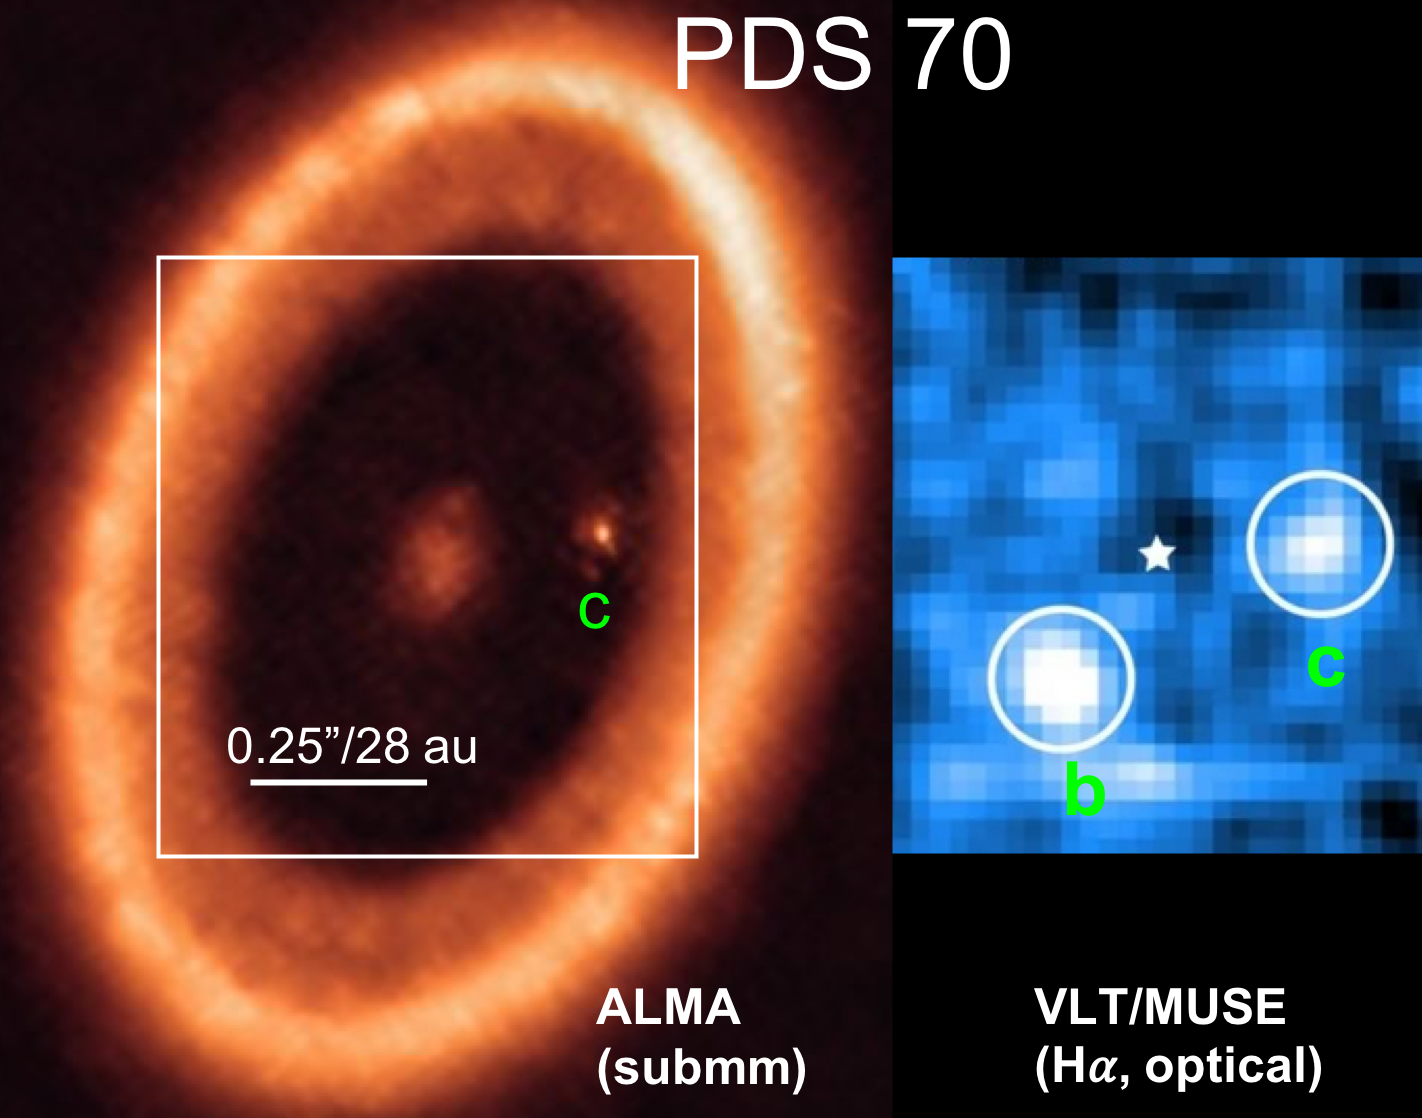
\includegraphics[width=\figwidth]{Figure_Chap1/Currie2022_Figure7a.png}
    \caption[Images du système PDS 70.]{Image dans la gamme de longueur d'onde millimétrique obtenue sur le télescope ALMA (Atacama Large Millimeter/Submillimiter Array) \citep{benisty2021}, mettant en évidence le disque protoplanétaire et sa cavité de PDS 70 ainsi que le compagnon PDS 70 c et son disque circumplanétaire. Image dans la raie \ha~obtenue sur l'instrument MUSE du VLT \citep{haffert2019} sur laquelle les deux compagnons sont détectés. Le champ de vue de cette dernière correspond au champ de vue délimité par le rectangle blanc sur l'image de gauche. La composition d'images est tirée de \cite{currie2022a}.}
    \label{fig:PDS70Image}
\end{figure}

Les deux compagnons sont localisés dans la cavité du disque, à une séparation de $180 \,$mas (demi-grand axe de $20 \,$ua) et $240 \,$mas (demi-grand axe de $34 \,$ua) respectivement pour PDS 70 b et c \citep{wang2021}. Leur masse est estimée à $1 - 10 \, \MJ$ \citep{wang2021, haffert2019}. Les différentes méthodes exposées dans la partie précédente ont été utilisées dans plusieurs études pour estimer le taux d'accrétion. Celui-ci est trouvé dans l'intervalle $1-10 \times 10^{-8} \, \MJ.\text{yr}^{-1}$ pour les deux planètes \citep{wagner2018, haffert2019, aoyama2019, thanathibodee2019, hashimoto2020}. Au vu de ces connaissances, il s'agit à l'heure actuelle de la première détection confirmée de protoplanète.

% contraste de pds70 : $\sim 2.10^{-2}$ \citep{hashimoto2020} avec variation de $10\%$ à cause de l'étoile
Le rapport de flux (contraste) entre la planète b et l'étoile centrale est estimé à $\sim 1.10^{-3}$ \citep{wagner2018, zhou2021}. Cela induit un signal de phase valant $\sim 0,06\degree$ lors de mesures interférométriques. Ainsi, les développements de \ac{FIRST}, dont le travail de ma thèse fait partie, sont menés pour atteindre de telles sensibilités afin de détecter le signal d'une protoplanète.

Les mesures de largeur à $10\%$, \Wd, des raies d'émission \ha~de \cite{haffert2019} sont de $\sim 224 \pm 24 \, \text{km}.\text{s}^{-1}$ et $\sim 186 \pm 35 \, \text{km}.\text{s}^{-1}$ pour les planètes b et c respectivement. Cela correspond à des largeurs spectrales de $0,49 \pm 0,05 \,$nm et de $0,41 \pm 0,08 \,$nm, respectivement. Ainsi, pour obtenir $6$ points de mesure (pour être bien au-dessus du critère de Shanon) d'une raie d'émission \ha~de largeur égale à $200 \, \text{km}.\text{s}^{-1}$, un instrument doit disposer d'un pouvoir de résolution spectrale égal à $R = 9\,000$. Avec le nouveau concept de spectrographe récemment intégré à \ac{FIRSTv2} (voir la section~\ref{sec:InstruSpectro} à ce sujet), nous disposons d'un pouvoir de résolution égal à $3\,400$. Ce pouvoir de résolution permet de mesurer au moins $6$ points de raies d'émission de largeur supérieur à $\sim 529 \, \text{km}.\text{s}^{-1}$. Il est ainsi prévu que nous n'exploitions pas la mesure de la largeur \Wd~de la raie d'émission lors de futures observations, mais seulement l'intensité de celle-ci. Mais lorsque la sensibilité de l'instrument sera suffisante, la résolution spectrale de l'instrument pourra être augmenté (d'un facteur $\sim 2,6$) afin de permettre la mesure de la largeur \Wd~et contraindre le taux d'accrétion de la protoplanète observée.

% Des forts taux d'accrétion favorisent CA
% It should be noted that the community remains unsure of the formation mechanism of the PDS 70 planets. Bright and widely separated exoplanets such as the HR 8799 planets are often thought to have been formed by disk instability (Boss 2011). However, due to the presence of accretion on the PDS 70 planets, core accretion is one of the potential scenarios (as for the planets in our own solar system, e.g. Nesvorny, 2018). In the case of planets formed by core accretion, the accretion rate is expected to be at least as high as what is observed in the PDS 70 planets. The closer in time they are to the run-away accretion phase (that is when the planets acquire a critical mass to clear the gas and create a gap in the transitional disk), the more material the planets accrete (Fig. 1 top panel)
